\let\negmedspace\undefined
\let\negthickspace\undefined
\documentclass[journal]{IEEEtran}
\usepackage[a5paper, margin=10mm, onecolumn]{geometry}
\usepackage{tfrupee} 

\setlength{\headheight}{1cm}
\setlength{\headsep}{0mm}

\usepackage{gvv-book}
\usepackage{gvv}
\usepackage{cite}
\usepackage{amsmath,amssymb,amsfonts,amsthm}
\usepackage{algorithmic}
\usepackage{graphicx}
\usepackage{textcomp}
\usepackage{xcolor}
\usepackage{txfonts}
\usepackage{listings}
\usepackage{enumitem}
\usepackage{mathtools}
\usepackage{gensymb}
\usepackage{comment}
\usepackage[breaklinks=true]{hyperref}
\usepackage{tkz-euclide} 
\usepackage{listings}

\def\inputGnumericTable{}                                 
\usepackage[latin1]{inputenc}                                
\usepackage{color}                                            
\usepackage{array}                                            
\usepackage{longtable}                                       
\usepackage{calc}                                             
\usepackage{multirow}                                         
\usepackage{hhline}                                           
\usepackage{ifthen}                                           
\usepackage{lscape}

\title{\textbf{2.3.9}}
\author{\textbf{EE25BTECH11006 - ADUDOTLA SRIVIDYA}}
\date{August 29, 2025}

\begin{document}

\maketitle

\section*{\textbf{Question}}
If vectors $\vec{a}$ and $\vec{b}$ are such that $|\vec{a}| = \frac{1}{2}$, $|\vec{b}| = \frac{4}{\sqrt{3}}$ and $|\vec{a} \times \vec{b}| = \frac{1}{\sqrt{3}}$, then find $\vec{a} \cdot \vec{b}$.

\section*{\textbf{Solution}}
We know that
\begin{align}
|\vec{a} \times \vec{b}| &= |\vec{a}||\vec{b}|\sin\theta \\
\vec{a} \cdot \vec{b} &= |\vec{a}||\vec{b}|\cos\theta
\end{align}
where $\theta$ is the angle between $\vec{a}$ and $\vec{b}$.

\noindent
Substitute the values:
\begin{align}
\frac{1}{\sqrt{3}} &= \left(\frac{1}{2}\right)\left(\frac{4}{\sqrt{3}}\right)\sin\theta \\
\frac{1}{\sqrt{3}} &= \frac{2}{\sqrt{3}} \sin\theta \\
\sin\theta &= \frac{1}{2}
\end{align}

Thus,
\begin{align}
\theta = 30^\circ \quad \text{or} \quad 150^\circ
\end{align}

\noindent
Now,
\begin{align}
\vec{a} \cdot \vec{b} &= |\vec{a}||\vec{b}|\cos\theta \\
&= \left(\frac{1}{2}\right)\left(\frac{4}{\sqrt{3}}\right)\cos\theta \\
&= \frac{2}{\sqrt{3}}\cos\theta
\end{align}

\noindent
So, the possible values are:
\begin{align}
\vec{a} \cdot \vec{b} &= \frac{2}{\sqrt{3}} \cdot \frac{\sqrt{3}}{2} = 1 \quad (\theta = 30^\circ) \\
\vec{a} \cdot \vec{b} &= \frac{2}{\sqrt{3}} \cdot \left(-\frac{\sqrt{3}}{2}\right) = -1 \quad (\theta = 150^\circ)
\end{align}

\centering
Therefore, $\vec{a} \cdot \vec{b} = \pm 1$.
\newpage
\begin{figure}[H]
    \centering
    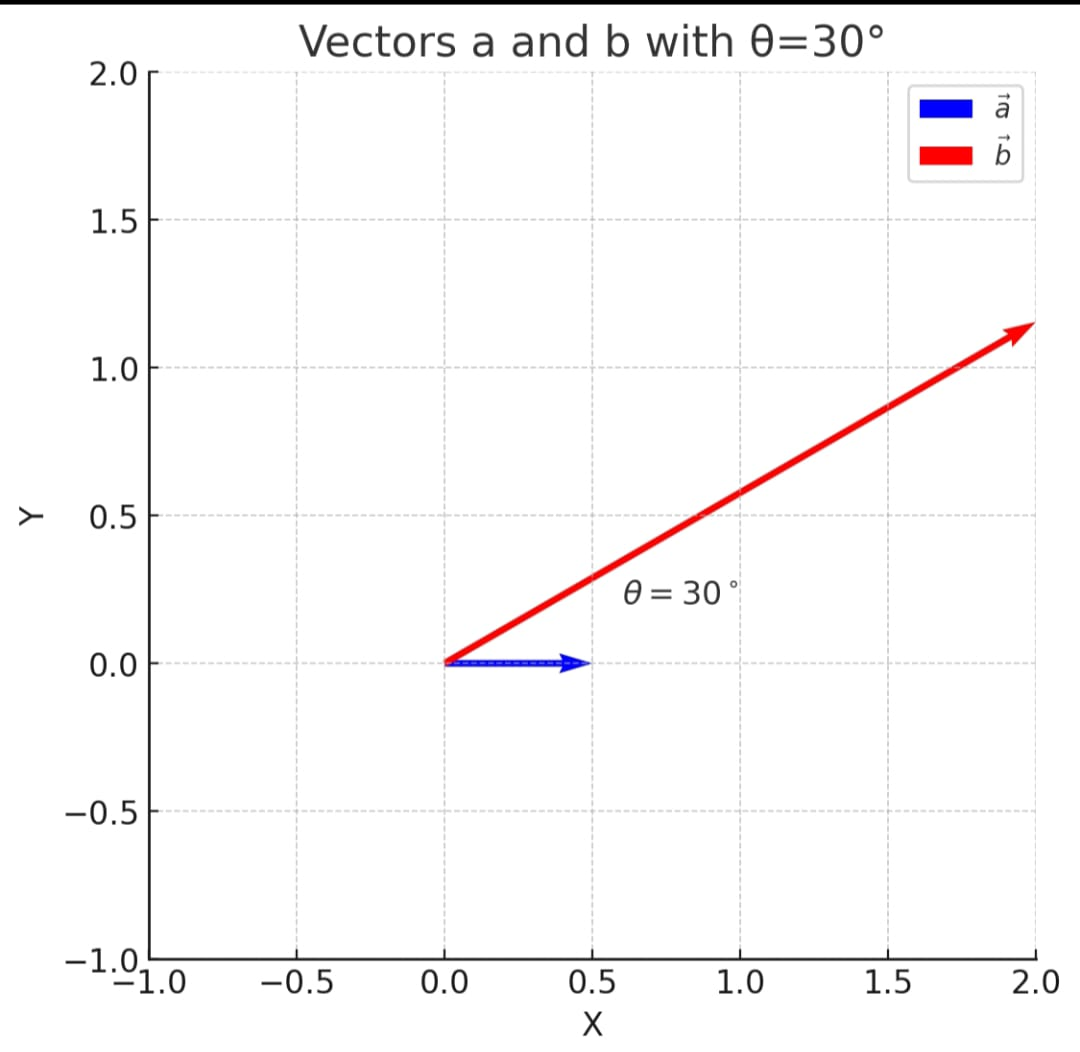
\includegraphics[width=0.7\columnwidth]{figs/fig2.3.9.jpeg}
    \caption{Vectors $\vec{a}$ and $\vec{b}$ with angle $\theta$}
    \label{fig:placeholder}
\end{figure}

\end{document}